% presentation.tex
% Beamer template (français) pour une présentation de projet (structure en 4 parties)
\documentclass[11pt]{beamer}

% Langue et encodage
\usepackage[T1]{fontenc}
\usepackage[utf8]{inputenc}
\usepackage[french]{babel}
\usepackage{lmodern}
\usepackage{microtype}
% Avoid requests for sans small-caps (Latin Modern Sans has no sc shape)
\renewcommand{\scshape}{\upshape}
\usepackage{graphicx}
\usepackage{amsmath,empheq}
\usepackage{hyperref}
\usepackage{csquotes}
\usepackage[backend=biber, style=numeric]{biblatex}
\addbibresource{biblio.bib}
\hypersetup{pdfauthor={R. Vivant}, pdftitle={Automated Calibration of Physical Models}}

% Thème et couleurs
\usetheme{Madrid}            % thème clair et professionnel
\usecolortheme{seagull}
\setbeamertemplate{navigation symbols}{} % supprime icônes de navigation
% Avoid requesting small caps in sans fonts (Latin Modern Sans doesn't provide sc);
% force upright (no small caps) for title/frametitle/author to prevent font shape warnings.
\setbeamerfont{frametitle}{series=\bfseries,shape=\upshape}
\setbeamerfont{title}{series=\bfseries,shape=\upshape}
\setbeamerfont{author}{series=\mdseries,shape=\upshape}

% Couleurs personnalisées
\definecolor{accent}{RGB}{0,102,153}
\setbeamercolor{frametitle}{bg=accent, fg=white}
\setbeamercolor{title}{bg=white, fg=accent}
\setbeamercolor{structure}{fg=accent}

% Infos du titre
\title[Automated Calibration]{Automated Calibration of Physical Models for Musical Instruments}
\author[R. M. Vivant]{Rodolphe Milton Vivant}
\institute[Ufr Mathématiques et Informatique de Strasbourg]{Master 2 — Projet}
\date{\today}

% En-tête / pied de page
\setbeamertemplate{footline}{
    \leavevmode%
    \hbox{%
    \begin{beamercolorbox}[wd=.65\paperwidth,ht=2.5ex,dp=1ex,left]{author in head/foot}%
        \hspace{1em}\insertshortauthor{} — \insertshortinstitute
    \end{beamercolorbox}%
    \begin{beamercolorbox}[wd=.35\paperwidth,ht=2.5ex,dp=1ex,right]{date in head/foot}%
        \insertshortdate{}\hspace{1em}
    \end{beamercolorbox}}%
    \vskip0pt%
}
\setbeamertemplate{headline}{}

% Commandes utiles
\newcommand{\slideTitle}[1]{\begin{frame}\frametitle{#1}}

% Document
\begin{document}

% Page de titre
\begin{frame}[plain]
    \titlepage
    % Trois logos sous la page de titre — adaptez les chemins/noms de fichiers
    \vfill
    \begin{center}
        
\includegraphics[height=2.5cm]{Images/inria_logo.png}\hspace{0.0em}%
        
\includegraphics[height=2.5cm]{Images/modartt_logo.png}\hspace{0.0em}%
        
\includegraphics[height=1.6cm]{Images/logo_irma.png}
    \end{center}
    \vspace{0.8em}
    % Si vous avez un logo : \includegraphics[height=1.5cm]{logo.png}
\end{frame}

% Plan
\begin{frame}
    \frametitle{Plan}
    \tableofcontents
\end{frame}

% Section 1
\section{Objectives and Context}
\slideTitle{Context}
\begin{itemize}
    \item Automatically adjust parameters of physical models to match target sounds of reed instruments.
    \item Joint collaboration between IRMA and Modartt.
    \item Modartt \footnotemark is a French company specialized in the development of artistic and technological application software (PIANOTEQ model).
\end{itemize}

\footnotetext{
{\footnotesize \cite{Modartt}
\url{https://www.modartt.com/}}
}
\end{frame}

\slideTitle{Objectives}
In JAX framework:
\begin{itemize}
    \item Implement a discontinuous Galerkin discretisation of the mixt form of the wave and numerically solve it.
    \item Implement the coupling with an ODE and the boundary conditions of a reed instrument.
    \item Compute the gradient with respect to all parameters.
\end{itemize}
\end{frame}

\section{Theoritical Aspects}
\slideTitle{Reed Instruments}
\begin{itemize}
    \item \footnotemark[1] Reed : thin, flexible lamina mounted at the mouthpiece or at the entrance of an air column resonator.
    \item \footnotemark[2] When subjected to a pressure difference $\rightarrow$ generates self-sustained oscillations (sound).
\end{itemize}
            
\begin{columns}[T]
    \begin{column}{0.5\textwidth}
        \begin{itemize}
            \item Two principal categories of reed instruments:
                \begin{itemize}
                    \item Free reeds (harmonicas, accordions, ...).
                    \item Beating reeds (clarinets, saxophones, ...).
                \end{itemize}
        \end{itemize}
    \end{column}
    \begin{column}{0.5\textwidth}
        \centering
        \vspace{-1ex}
        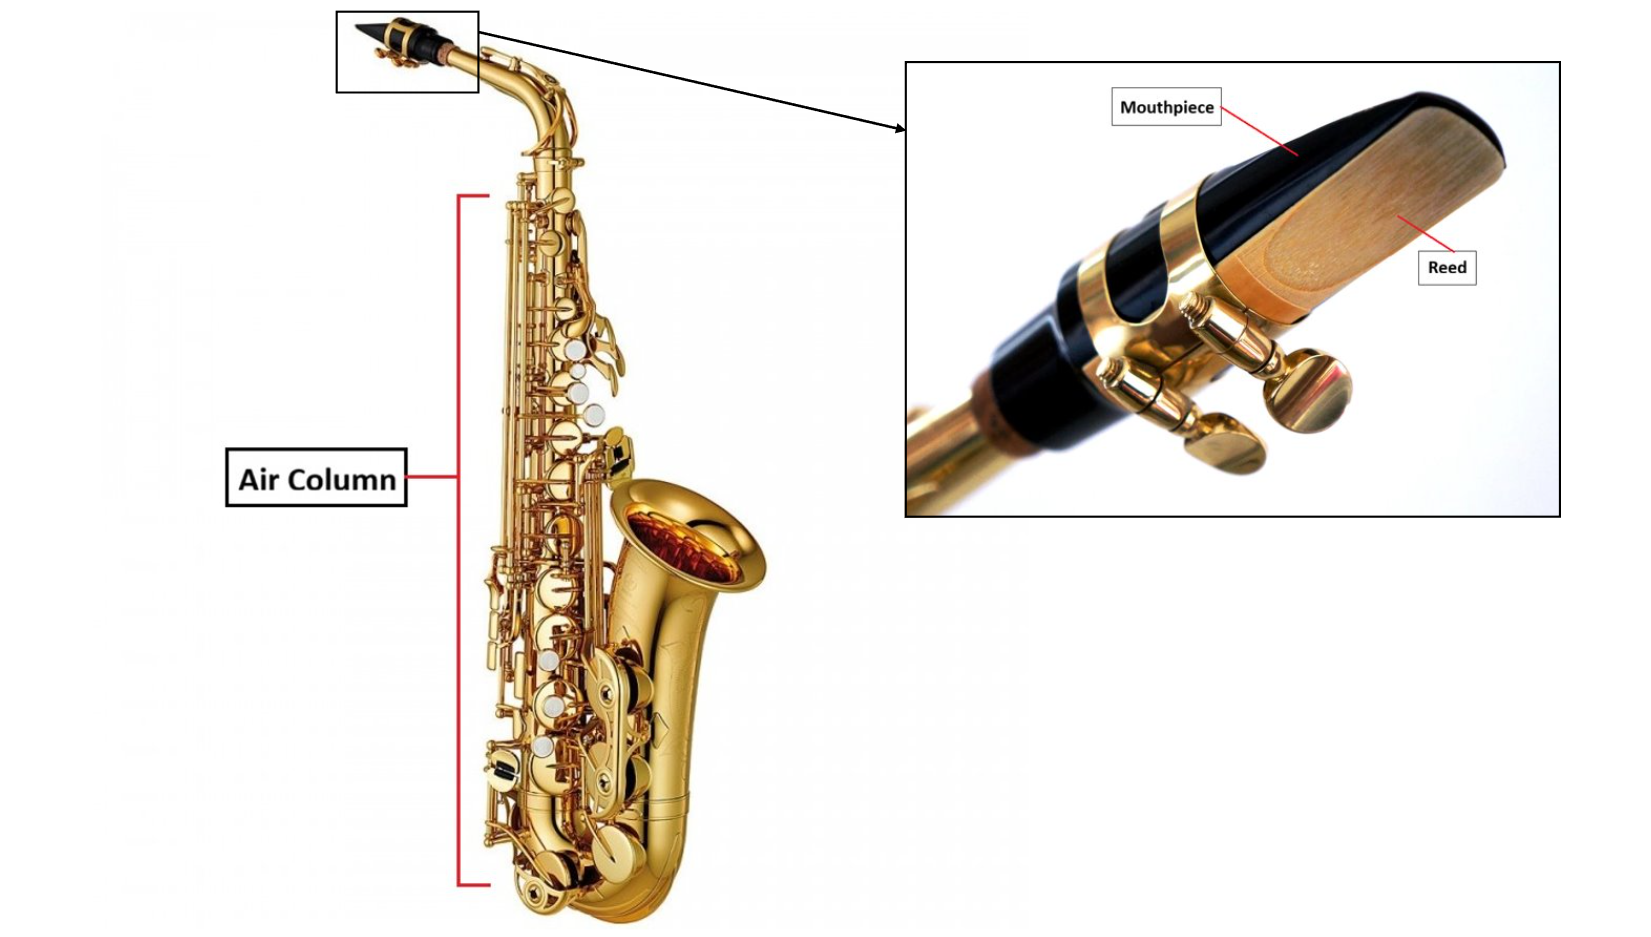
\includegraphics[width=\linewidth,keepaspectratio]{Images/reed_column.png} 
        \par\smallskip
        \scriptsize Example of a saxophone reed and mouthpiece.
        \label{fig:sax_reed}
    \end{column}
\end{columns}
\footnotetext[1]{
{\footnotesize \cite{Universalis_Anche} 
Encyclopædia Universalis, "Anche (instrument de musique)".
}
}
\footnotetext[2]{
{\footnotesize \cite{chaigne:hal-05370840}
Chaigne, A. (2010). "Physical models of musical instruments". HAL.
}
}
\end{frame}

\slideTitle{Physical Model}

\small
\noindent\begin{minipage}[t]{\linewidth}
\begin{subequations}
\begin{empheq}[left=\empheqlbrace]{align}
    \frac{S(x)}{c S^\ast}\,\partial_t p(x,t) + \partial_x v(x,t) &= 0\\[4pt]
    \frac{S^\ast}{c S(x)}\,\partial_t v(x,t) + \partial_x p(x,t) &= 0 \\[4pt]
    Z^\ast_T\,\partial_t \phi + \sqrt{\alpha}\,p(L,t) &= 0 \\[4pt]
    -\frac{\beta}{Z^\ast_T}\,p(L,t) + v(L,t) + \sqrt{\alpha}\,\phi &= 0 \\[4pt]
    -v(0,t) + \zeta \ell(y)\,F(\gamma - p(0,t)) + \varepsilon\frac{\kappa}{\omega_r}\,\partial_t y &= 0 \\[6pt]
    \frac{1}{\omega_r^2}\,\partial_{tt} y + \frac{1}{Q_r\omega_r}\,\partial_t y + y - 1 
    &= \varepsilon(\gamma - p(0,t)) 
\end{empheq}
\end{subequations}
\end{minipage}
\end{frame}

\slideTitle{Physical Model}
\noindent\begin{minipage}[t]{\linewidth}
\begin{subequations}
\begin{empheq}[left=\empheqlbrace]{align}
    \frac{S(x)}{c S^\ast}\,\partial_t p(x,t) + \partial_x v(x,t) &= 0\label{eq:1a} \\[4pt]
    \frac{S^\ast}{c S(x)}\,\partial_t v(x,t) + \partial_x p(x,t) &= 0\label{eq:1b}
\end{empheq}
\end{subequations}
\end{minipage}
\begin{itemize}
    \item Equations \eqref{eq:1a} and \eqref{eq:1b}: wave propagation (pressure and acoustic volume velocity)in a variable section tube. \footnotemark[1]
    \item $S(x)$: cross-section area, $c$: speed of sound, $S^\ast$: reference cross-section area.
\end{itemize}
\footnotetext[1]{
{\scriptsize \cite{MAMAMIA2024}
Michel-Dansac, V., Thibault, A., Franck, E., Chabassier, J., Navoret, L. (2024). "Automated Calibration of Physical Models for Reed Instruments". MAMAMIA 2024.
}
}
\end{frame}

\slideTitle{Physical Model}
\begin{itemize}
    \item At the outlet $x=L$ : Influence of exterior environment through a condition
    of radiation impedance \footnotemark[1],
\end{itemize}
\noindent\begin{minipage}[t]{\linewidth}
\begin{subequations}
\begin{empheq}[left=\empheqlbrace]{align}
    &Z^\ast_T\,\partial_t \phi + \sqrt{\alpha}\,p(L,t) = 0 \label{eq:1c} \\[4pt]
    -&\frac{\beta}{Z^\ast_T}\,p(L,t) + v(L,t) + \sqrt{\alpha}\,\phi = 0 \label{eq:1d} 
\end{empheq}
\end{subequations}
\end{minipage}
\begin{itemize}
    \item \ref{eq:1c} : time evolution of the boundary variable $\phi(t)$. (Euler Explicit or RK2 time integration).
    \item \ref{eq:1d} enforces a dynamic impedance relation between pressure and velocity (link to DG).
    \item $Z_T^\ast$: characteristic impedance, $\alpha,\beta$: parameters related to the acoustic load.
\end{itemize}

\footnotetext[1]{
{\footnotesize \cite{thibault}
Thibault, Alexis (2023), \emph{Mod{\'e}lisation, analyse et simulation de l'acoustique dissipative dans les tubes poreux ou rugueux : application aux instruments {\`a} vent}}
}
\end{frame}

\slideTitle{Physical Model}
\noindent\begin{minipage}[t]{\linewidth}
\begin{subequations}
\begin{empheq}[left=\empheqlbrace]{align}
    -&v(0,t) + \zeta \ell(y)\,F(\gamma - p(0,t)) + \varepsilon\frac{\kappa}{\omega_r}\,\partial_t y = 0 \label{eq:1e} \\[6pt]
    &\frac{1}{\omega_r^2}\,\partial_{tt} y + \frac{1}{Q_r\omega_r}\,\partial_t y + y - 1 
    = \varepsilon(\gamma - p(0,t)) \label{eq:1f}
\end{empheq}
\end{subequations}
\end{minipage}
\begin{itemize}
    \item Equations \eqref{eq:1e} and \eqref{eq:1f}: effects of the instrumental player at the input boundary.
    \item \(\gamma\) denotes the mouth pressure, \(\omega_r = 2\pi f_r\) the resonance frequency of the lips or 
    reed, \(Q_r\) quality factor , \(\zeta\) a dimensionless stiffness parameter, and \(\kappa\) the reed flow 
    efficiency, \(\varepsilon = \pm 1\).
    \item $F$: nonlinear function modeling the airflow through the reed channel. $F(\Delta p) = \sqrt{\Delta p}sign(\Delta p)$
\end{itemize}
\end{frame}



% Section 2
\section{Methods}
\subsection{Discontinuous Galerkin Method}

\slideTitle{Discontinuous Galerkin Method}

\begin{itemize}
    \item \footnotemark Numerical method for the spatial discretization of partial differential equations.
    \item We consider a scalar conservation law:
    \begin{equation}\label{eq:transport}
        \partial_t u(x,t) + \partial_x F\big(u(x,t)\big) = 0,
        \qquad u : \Omega \times [0,T] \rightarrow \mathbb{R}.
    \end{equation}
    \item $F : \mathbb{R} \rightarrow \mathbb{R}$ denotes the flux function.
    \item Time discretization using an explicit Euler scheme with time step $\Delta t$.
    \item At time $t^n = n\Delta t$, we approximate $u(x,t^n)$ by $u^n(x)$:
    \begin{equation}
        u^{n+1}(x) = u^n(x) - \Delta t\, \partial_x F\big(u^n(x)\big).
    \end{equation}
\end{itemize}
\footnotetext{
\footnotesize \cite[Section~2]{HesthavenWarburton2008}
Hesthaven and Warburton (2008), \emph{Nodal Discontinuous Galerkin Methods}, Section~4.5
}
\end{frame}


\slideTitle{Discontinuous Galerkin Method (cont.)}

Assume that $u_h^n$ (approximation of $u(\cdot,t^n)$) is known.
\begin{itemize}
    \item Partition the domain $\Omega$ into $K$ non-overlapping elements $\{\Omega_k\}$.
    \item On each element $\Omega_k$, approximate the solution by
    \[
        u_h^n|_{\Omega_k} = u_k^n(x) = \sum_j \alpha_{k,j}^n \, \phi_j(x),
    \]
    where $\{\phi_j\}$ is a local polynomial basis.
    \item Enforce the weak formulation on each element:
    \begin{equation}
        \int_{\Omega_k} u_k^{n+1}(x)\phi_i(x)\,dx
        =
        \int_{\Omega_k} u_k^n(x)\phi_i(x)\,dx
        -
        \Delta t
        \int_{\Omega_k} \partial_x F\big(u_k^n(x)\big)\phi_i(x)\,dx.
    \end{equation}

\end{itemize}
\end{frame}

\slideTitle{Discontinuous Galerkin Method (cont.)}
\begin{itemize}
    \item Integration by parts yields:
    \small
    \begin{equation}
        \begin{aligned}
        \sum_j \alpha_{k,j}^{n+1}
        \int_{\Omega_k} \phi_j(x)\phi_i(x)\,dx
        &= 
        \int_{\Omega_k} u_k^n(x)\phi_i(x)\,dx
        +\\
        &\Delta t\int_{\Omega_k} F\big(u_k^n(x)\big)\partial_x\phi_i(x)\,dx
        -
        \Delta t\left[ F(u_k^n)\phi_i \right]_{\partial\Omega_k}
        \end{aligned}
    \end{equation}
    \normalsize
    \item Define the local mass matrix
    $
        M_{ij} = \int_{\Omega_k} \phi_j(x)\phi_i(x)\,dx.
    $
    \item The local system (on each element $\Omega_k$) reads:
    \begin{equation}
        M\,\boldsymbol{\alpha}_k^{\,n+1} = \mathbf{b}_k^n,
    \end{equation}
    where $\mathbf{b}_k$ depends only on $u_k^n$ and numerical fluxes.
\end{itemize}
\end{frame}


\subsection{DG in our context}

\slideTitle{DG in our context}

\begin{itemize}
    \item From the general expression : 
    \small
    \begin{equation}
        \mathbf{C}(x)\,\partial_t \mathbf{u}
        +
        \partial_x \big( \mathbf{A}\mathbf{u} \big)
        = 0,
    \end{equation}
    \normalsize
    where
    \scriptsize
    \[
        \mathbf{u} =
        \begin{pmatrix}
        p \\
        v
        \end{pmatrix},
        \quad
        \mathbf{C}(x) =
        \begin{pmatrix}
        \dfrac{S(x)}{cS^*} & 0 \\
        0 & \dfrac{S^*}{cS(x)}
        \end{pmatrix},
        \quad
        \mathbf{A} =
        \begin{pmatrix}
        0 & 1 \\
        1 & 0
        \end{pmatrix}.
    \]
    \normalsize
    \item Initial conditions:
    \[
        p(x,0) = p_0(x), \qquad v(x,0) = v_0(x).
    \]
    \item The domain is partitioned into $N$ non-overlapping cells
    $K_j = [x_{j-1},x_j]$.
    \item Mixed formulation of the one-dimensional wave equation with variable cross-section:
\end{itemize}

\begin{equation}
\scriptsize
\int_{K_j} \mathbf{C}(x)\,\partial_t \mathbf{u}_h \cdot \boldsymbol{\phi}\,dx
-
\int_{K_j} \mathbf{A}\mathbf{u}_h \cdot \partial_x \boldsymbol{\phi}\,dx
+ \widehat{\mathbf{F}}_{j+\frac12}\cdot \boldsymbol{\phi}(x_j^-)
-
\widehat{\mathbf{F}}_{j-\frac12}\cdot \boldsymbol{\phi}(x_{j-1}^+)
= 0,
\normalsize
\end{equation}

\end{frame}

\subsubsection{Rusanov Flux}

\slideTitle{DG in our context -- Rusanov Flux}

\begin{itemize}
    \item At each interface $x_{j+\frac12}$, the Rusanov (local Lax--Friedrichs) flux is defined as
    \begin{equation}
        \widehat{\mathbf{F}}
        =
        \frac12
        \Big(
        \mathbf{F}(\mathbf{u}^-)
        +
        \mathbf{F}(\mathbf{u}^+)
        \Big)
        -
        \frac{\lambda_{j+\frac12}}{2}
        \Big(
        \mathbf{u}^+ - \mathbf{u}^-
        \Big).
    \end{equation}

    \item The eigenvalues of $\mathbf{C}^{-1}\mathbf{A}$ (non conservative approach / need to be fixed) are
    \[
        \lambda_{1,2} = \pm c
        \quad \Rightarrow \quad
        \lambda_{j+\frac12} = c.
    \]
\end{itemize}

\end{frame}

\subsubsection{Final Formulation}
\slideTitle{DG in out context/Final DG formulation}
For each element $K_j=(x_{j-1},x_j)$ and 
for each test function $w_p,w_v\in\mathbb P^k(K_j)$, 
the DG formulation of the mixed form of the wave equation reads :

\begin{equation}
\begin{aligned}
\int_{K_j} \frac{S(x)}{cS^\ast}\,
\partial_t p_h \, \phi_p \, dx
&-
\int_{K_j} v_h \, \partial_x \phi_p \, dx \\
&+
\widehat{v}_{j+\frac12}\, \phi_p(x_j^-)
-
\widehat{v}_{j-\frac12}\, \phi_p(x_{j-1}^+)
=0,
\end{aligned}
\label{eq:dg_wave_p}
\end{equation}

\begin{equation}
\begin{aligned}
\int_{K_j} \frac{S^\ast}{cS(x)}\,
\partial_t v_h \, \phi_v \, dx
&-
\int_{K_j} p_h \, \partial_x \phi_v \, dx \\
&+
\widehat{p}_{j+\frac12}\, \phi_v(x_j^-)
-
\widehat{p}_{j-\frac12}\, \phi_v(x_{j-1}^+)
=0.
\end{aligned}
\label{eq:dg_wave_v}
\end{equation}
\end{frame}

\subsection{Boundary Conditions}

\slideTitle{Boundary Conditions: ODE--PDE Coupling}

\begin{itemize}
    \item At the outlet $x=L$ : Influence of exterior environment through a condition
    of radiation impedance \footnotemark[1],
    
    \item As shown in equations \eqref{eq:1c} and \eqref{eq:1d} :
    \begin{equation}
    \begin{cases}
        Z^\ast_T\,\partial_t \phi(t)
        + \sqrt{\alpha}\, p(L,t) = 0,
        \\[0.3em]
        -\dfrac{\beta}{Z^\ast_T}\, p(L,t)
        + v(L,t)
        + \sqrt{\alpha}\,\phi(t) = 0.
    \end{cases}
    \end{equation}

    \item The first equation : time evolution of the boundary variable $\phi(t)$. (Euler Explicit or RK2 time integration).
    \item The second equation enforces a dynamic impedance relation between pressure and velocity (link to DG).
\end{itemize}
\footnotetext[1]{
{\footnotesize \cite{thibault}
Thibault, Alexis (2023), \emph{Mod{\'e}lisation, analyse et simulation de l'acoustique dissipative dans les tubes poreux ou rugueux : application aux instruments {\`a} vent}}
}
\end{frame}

\slideTitle{Boundary Conditions in Characteristic Variables}

\begin{itemize}
    \item Introduce characteristic variables at the boundary:
    \begin{align}
        w^+ = p + v,
        \qquad
        w^- = p - v.
    \end{align}

    \item Using the impedance condition, the incoming characteristic can be expressed as:
    \begin{align}
        \boxed{
        w^- =
        \frac{1-\frac{\beta}{Z^\ast_T}}
             {1+\frac{\beta}{Z^\ast_T}}\, w^+
        +
        \frac{2\sqrt{\alpha}}
             {1+\frac{\beta}{Z^\ast_T}}\,\phi(t)
        }
    \end{align}

    \item This formulation allows a natural implementation within the DG framework:
    only the incoming wave $w^-$ is imposed.
\end{itemize}
\end{frame}

\slideTitle{Simplified Model and Exact Solution ($S(x)= S^* =1$)}

\begin{itemize}
    \item System: 
    \begin{align}
    \partial_t p + c \partial_x v &= 0 \\
    \partial_t v + c \partial_x p &= 0,
    \end{align}
    with $c$ constant and $x \in [0,L], t \in [0,T], \text{initial data } p_0, v_0$.
    \item Characteristics: 
    $$w^+_{pde} = p+v, \quad w^-_{pde} = p-v$$ 
    satisfy
    \begin{align}
    \partial_t w^+_{pde} + c \partial_x w^+_{pde} &= 0 \\
    \partial_t w^-_{pde} - c \partial_x w^-_{pde} &= 0.
    \end{align}
    \item Solution along characteristics:
    $$w^+_{pde}(x,t) = w^+_0(x-ct), \quad w^-_{pde}(x,t) = w^-_0(x+ct).$$
\end{itemize}
\end{frame}

\slideTitle{Boundary at $x=L$}

\begin{itemize}
    \item Impedance-type BC at $x=L$ with auxiliary variable $\phi(t)$:
    \begin{align}
        &\partial_t \phi(t) + c_1\, (1+a) w^+_{pde}(L,t) + c_2\, \phi(t) = 0,\\
        &w^-_{\mathrm{ref}}(L,t) = a\, w^+_{pde}(L,t) + b\, \phi(t).
    \end{align}
    Coefficients:
    \[
    a=\frac{1-\dfrac{\beta}{Z_T^\ast}}{1+\dfrac{\beta}{Z_T^\ast}}, \quad
    b=\frac{2\sqrt{\alpha}}{1+\dfrac{\beta}{Z_T^\ast}}, \quad
    c_1=\frac{\sqrt{\alpha}}{2Z_T^\ast}, \quad
    c_2=c_1 b.
    \]
    \item Solve $\phi(t)$ (Euler explicit or RK2)
    \item $w^-_{\mathrm{ref}}(x,t)=w^-_{\mathrm{ref}}(L,t-\frac{L-x}{c})$
\end{itemize}
\end{frame}

\slideTitle{Reflected Wave and Reconstruction}

\begin{itemize}
    \item Total left-going characteristic: $$w^-(x,t)= w^-_{pde}(x,t) + w^-_\mathrm{ref}(x,t)= w^-_0(x+ct) + w^-_\mathrm{ref}(x,t)$$.
    \item Right-going characteristic: $$w^+(x,t) = w^+_{pde}(x,t) =  w^+_0(x-ct)$$.
    \item Final solution: $$p = (w^+ + w^-)/2, \quad v = (w^+ - w^-)/2$$.
\end{itemize}
\end{frame}


\section{DG's results}

\subsection{Result - Constant Cross-Section}
\slideTitle{Result - Constant Cross-Section}
    \begin{figure}[htbp]
        \centering
        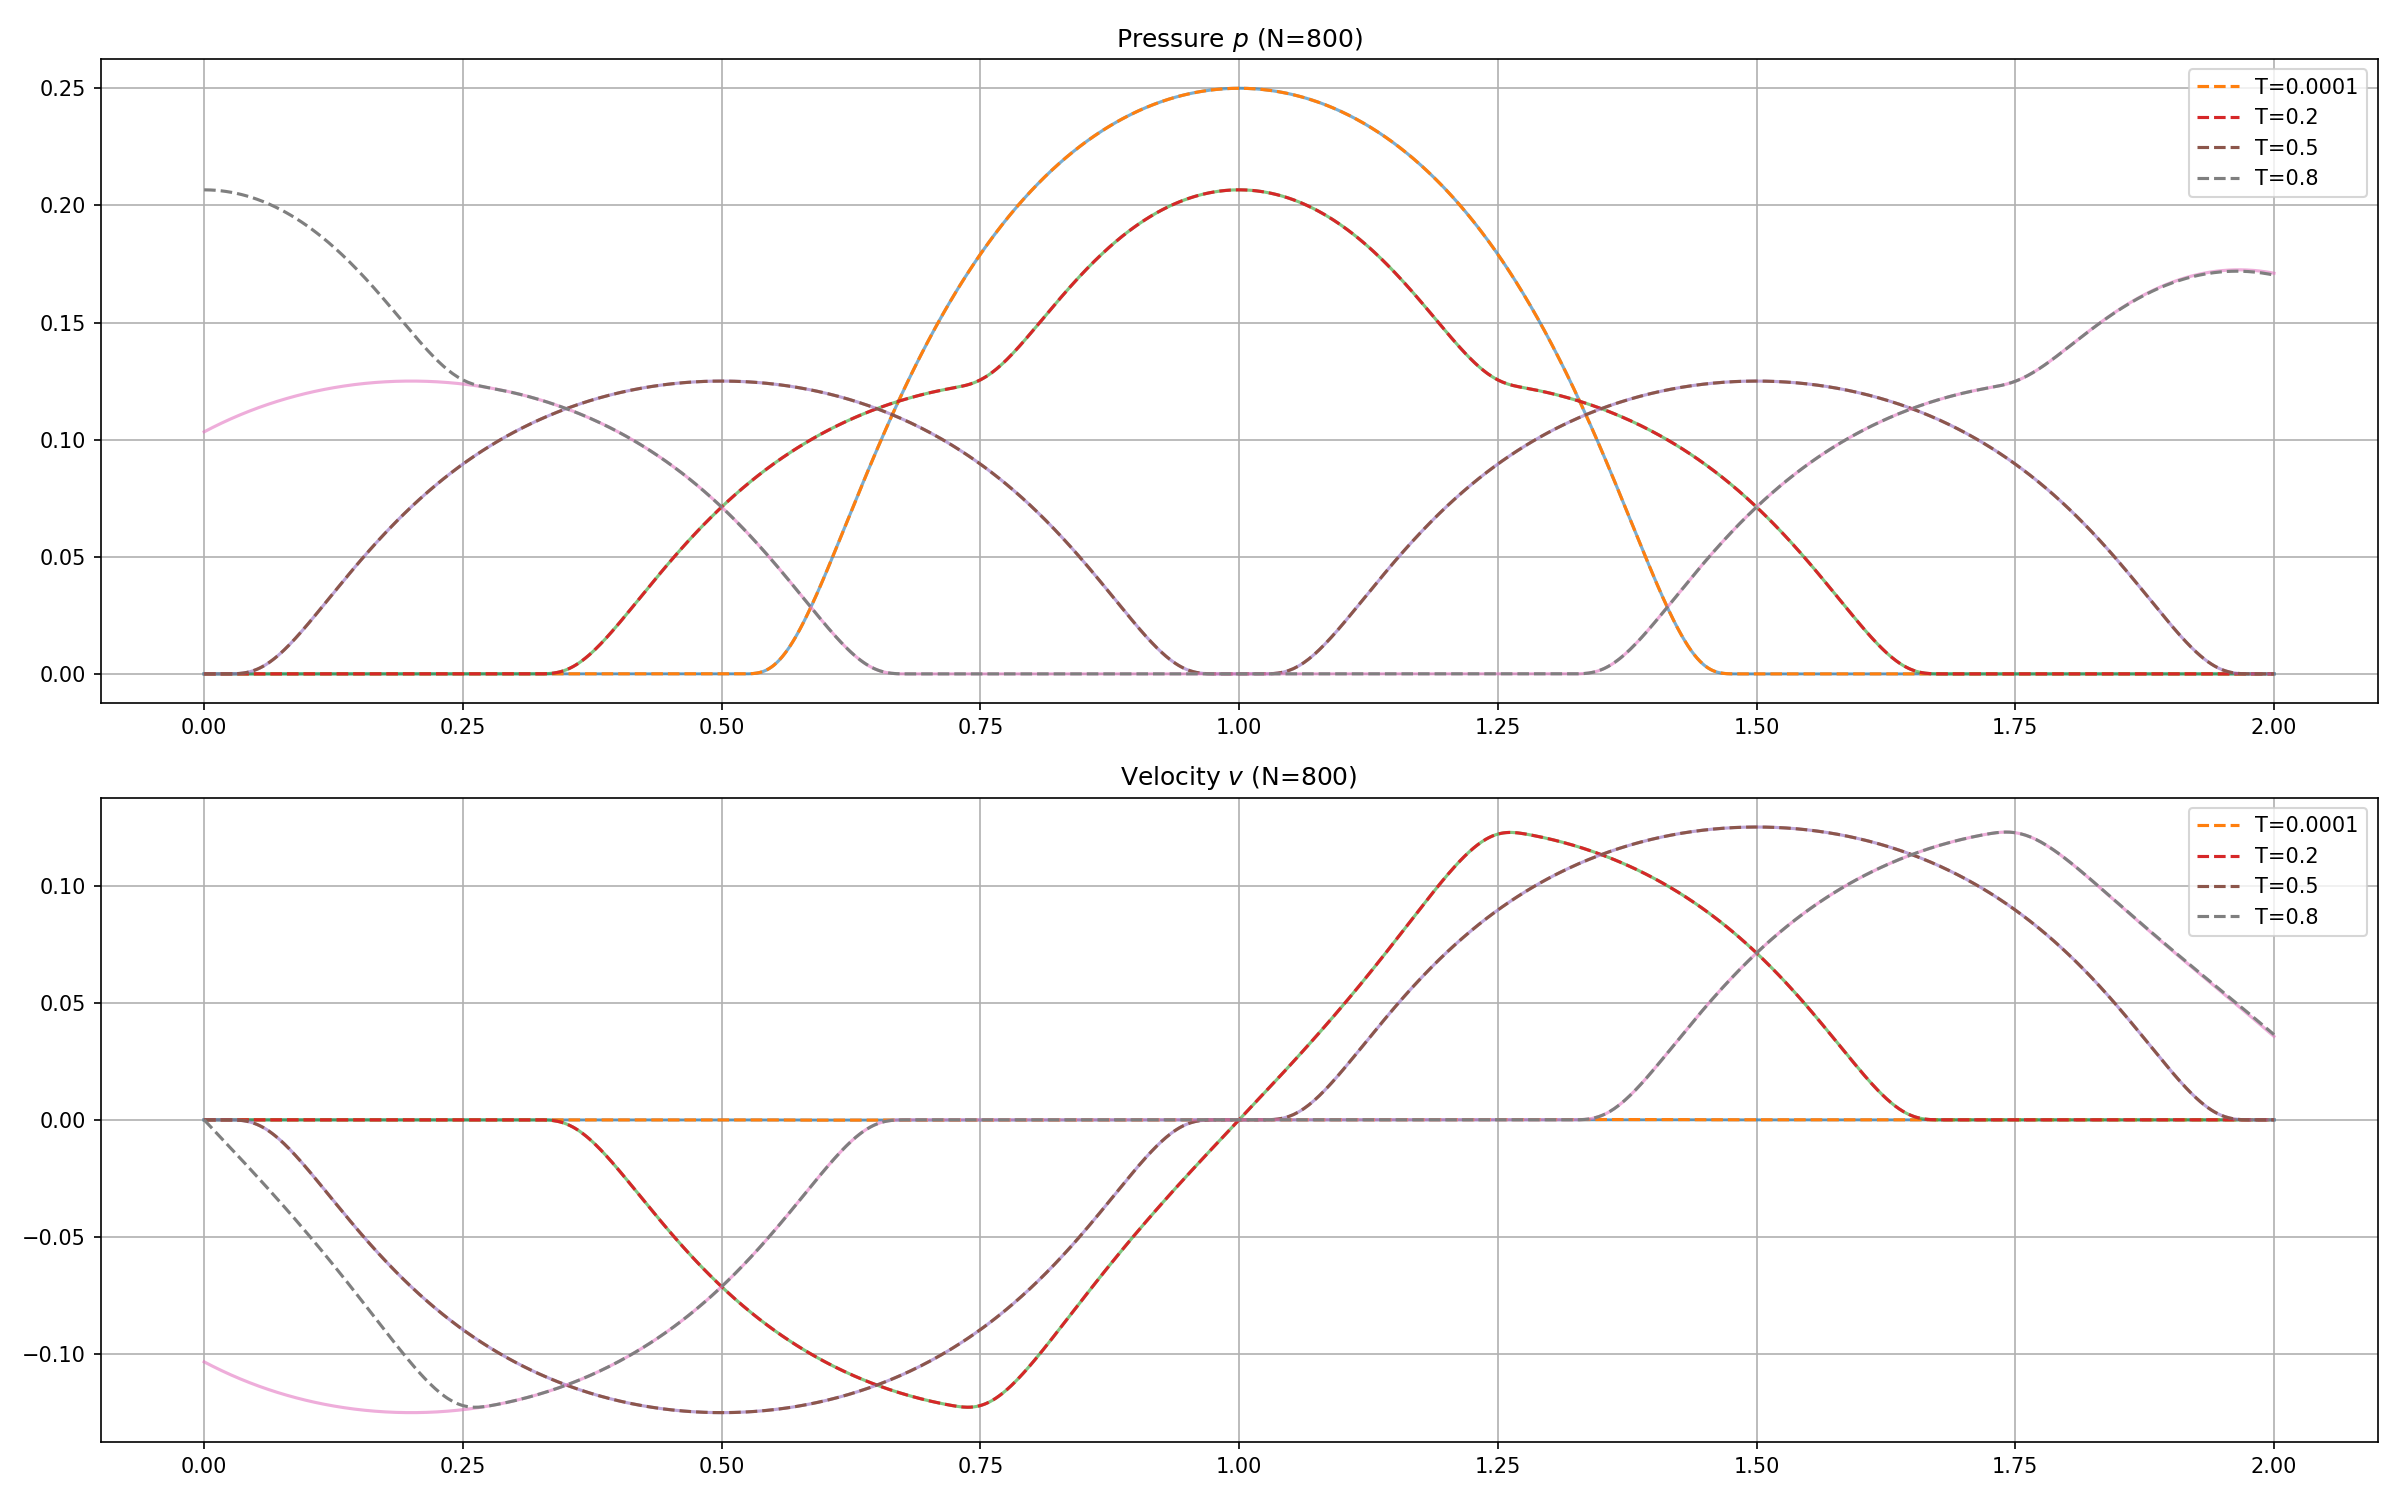
\includegraphics[width=0.65\textwidth]{Images/dg_solution_const_N800.png}
        \caption{DG numerical solutions constant cross-section.}
        \label{fig:dg_solution_const}
    \end{figure}
    \scriptsize
        \begin{equation}
            \begin{aligned}
            p_0(x) &=
            \begin{cases}
            \dfrac{\phi_0}{4}\,
            \exp\!\left(1 - \dfrac{1}{1-\xi(x)^2}\right),
            & \text{if } |\xi(x)| < 1, \\[1.2ex]
            0, & \text{otherwise}.
            \end{cases} \text{with } \xi(x) &= \dfrac{4(x - x_c)}{L} \\
            v_0(x) &= 0 \\
            \end{aligned}
        \end{equation}
    \normalsize
\end{frame}

\slideTitle{Convergence and Efficiency (Inside the domain)}

\begin{columns}[T]
    \begin{column}{0.5\textwidth}
        \centering
        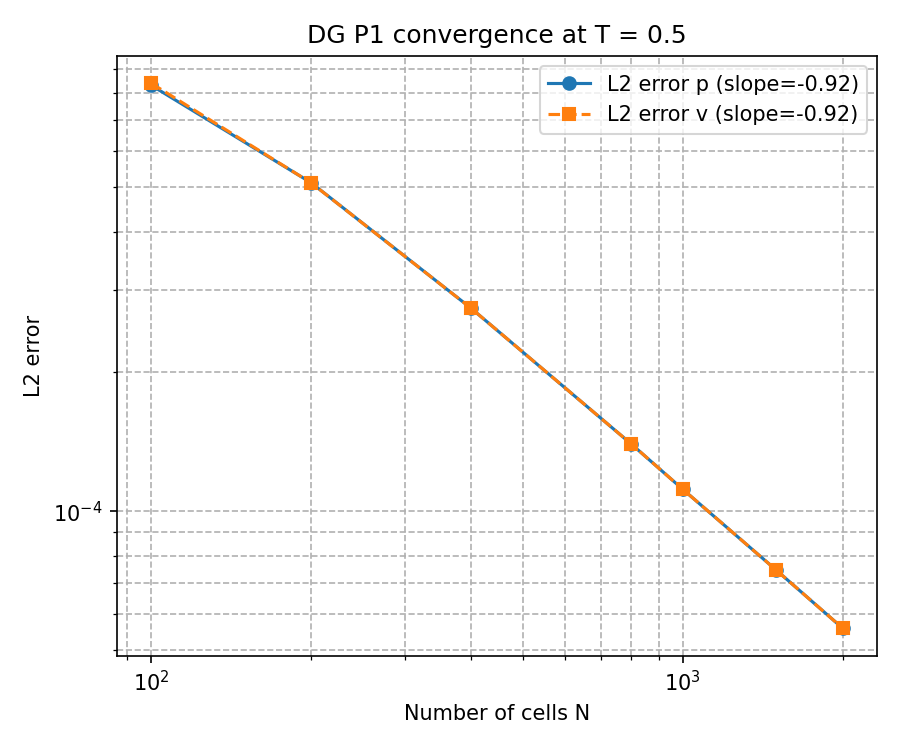
\includegraphics[width=0.7\linewidth]{Images/dg_convergence_T0.5_euler.png}
        
        {\scriptsize DG convergence with Explicit Euler scheme.}
    \end{column}

    \begin{column}{0.5\textwidth}
        \centering
        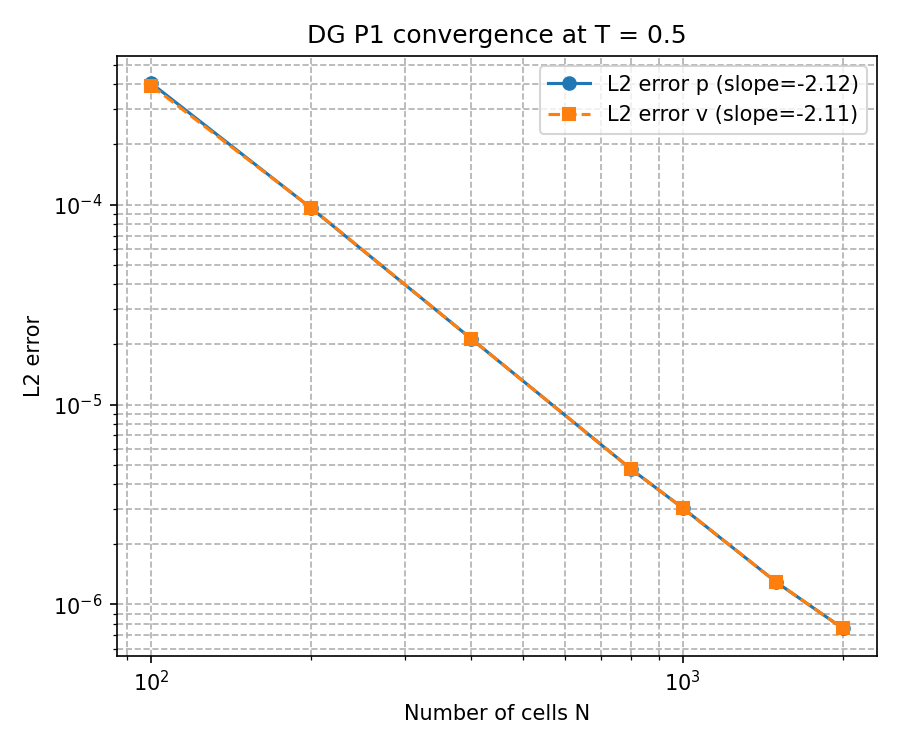
\includegraphics[width=0.7\linewidth]{Images/dg_convergence_T0.5_rk2.png}
        
        {\scriptsize DG convergence with Runge--Kutta second-order scheme.}
    \end{column}
\end{columns}

\vspace{0.3cm}
\scriptsize
\begin{itemize}
    \item \textbf{Spatial convergence:} order $d+1$ with polynomial degree $d$
    \footnotemark[1]
    \item \textbf{Temporal convergence:}
    \begin{itemize}
        \item Explicit Euler: first order
        \item Runge--Kutta 2: second order
    \end{itemize}
\end{itemize}
\normalsize

\footnotetext[1]{
{\footnotesize
\cite[Section~4.5]{HesthavenWarburton2008}
Hesthaven and Warburton (2008), \emph{Nodal Discontinuous Galerkin Methods}, Section~4.5
}
}

\end{frame}

\slideTitle{Convergence and Efficiency (At the boundary)}

\begin{columns}[T]
    \begin{column}{0.5\textwidth}
        \centering
        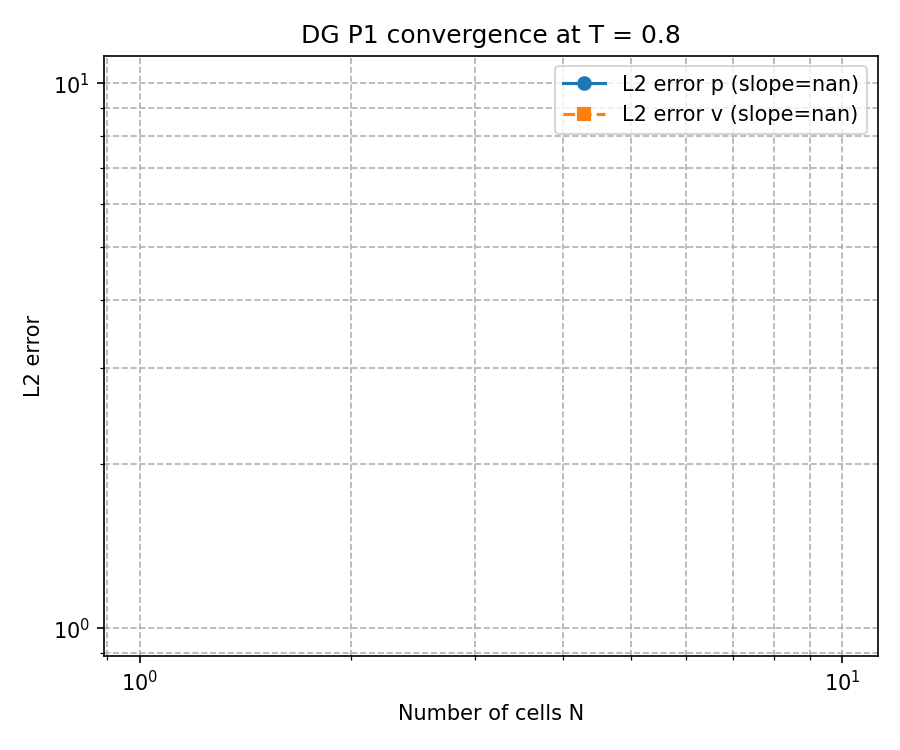
\includegraphics[width=0.7\linewidth]{Images/dg_convergence_T0.8_euler.png}
        
        {\scriptsize DG convergence with Explicit Euler scheme.}
    \end{column}

    \begin{column}{0.5\textwidth}
        \centering
        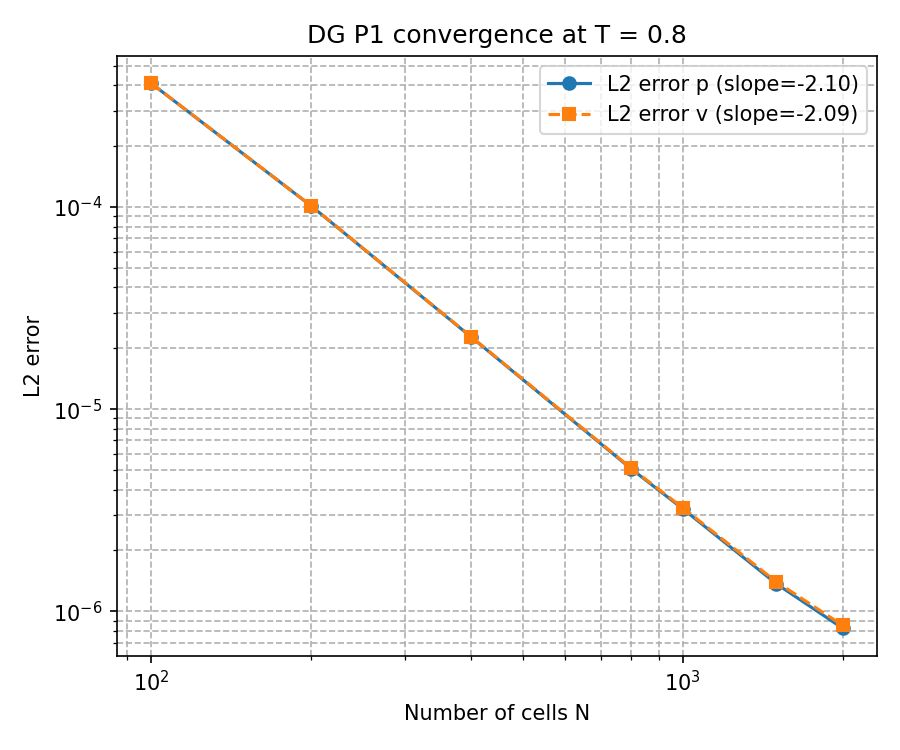
\includegraphics[width=0.7\linewidth]{Images/dg_convergence_T0.8_rk2.png}
        
        {\scriptsize DG convergence with Runge--Kutta second-order scheme.}
    \end{column}
\end{columns}

\vspace{0.3cm}
\scriptsize
\begin{itemize}
    \item \textbf{Spatial convergence:} order $d+1$ with polynomial degree $d$
    \footnotemark[1]
    \item \textbf{Temporal convergence:}
    \begin{itemize}
        \item Explicit Euler: first order
        \item Runge--Kutta 2: second order
    \end{itemize}
\end{itemize}
\normalsize

\footnotetext[1]{
{\footnotesize
\cite[Section~4.5]{HesthavenWarburton2008}
Hesthaven and Warburton (2008), \emph{Nodal Discontinuous Galerkin Methods}, Section~4.5
}
}

\end{frame}


\subsection{Result - Varying Cross-Section}               
\subsubsection{Examples of Cross-Section}
\slideTitle{Examples of Cross-Section}
\begin{columns}[T]
    \begin{column}{0.5\textwidth}
        \begin{figure}[htbp]
            \centering
            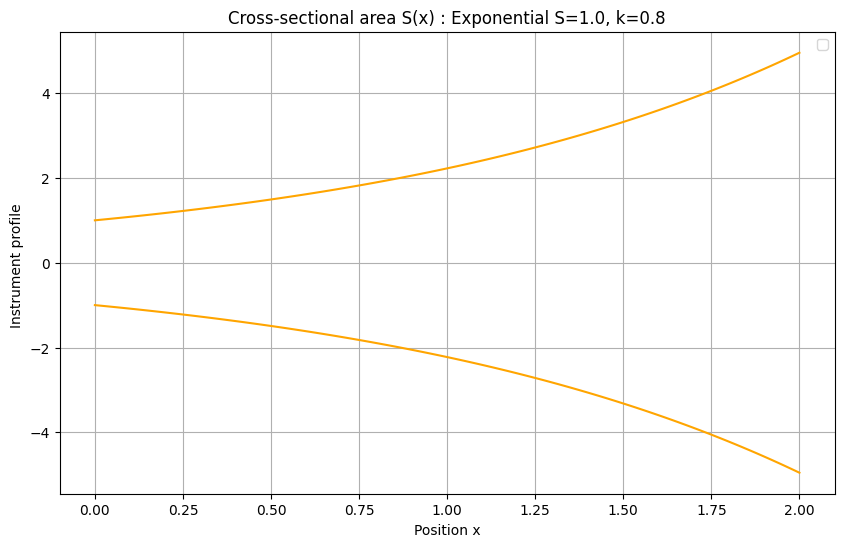
\includegraphics[width=\linewidth]{Images/exp_profile.png}
            \caption{Exponential cross-section $S(x) = S_0 e^{kx}$.}
            \label{fig:exp_profile}
        \end{figure}
    \end{column}
    \begin{column}{0.5\textwidth}
        \begin{figure}[htbp]
            \centering
            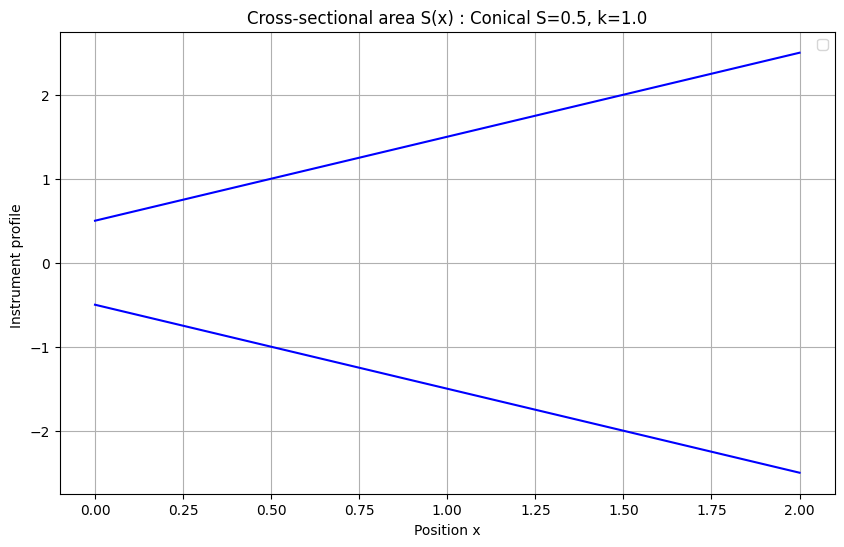
\includegraphics[width=\linewidth]{Images/cone_profile.png}
            \caption{Conical cross-section $S(x) = S_0 + kx$.}
            \label{fig:cone_profile}
        \end{figure}
    \end{column}
\end{columns}


\end{frame}
\subsubsection{Results}
\slideTitle{Result - Exponential Cross-Section}
\begin{figure}[htbp]
    \centering
    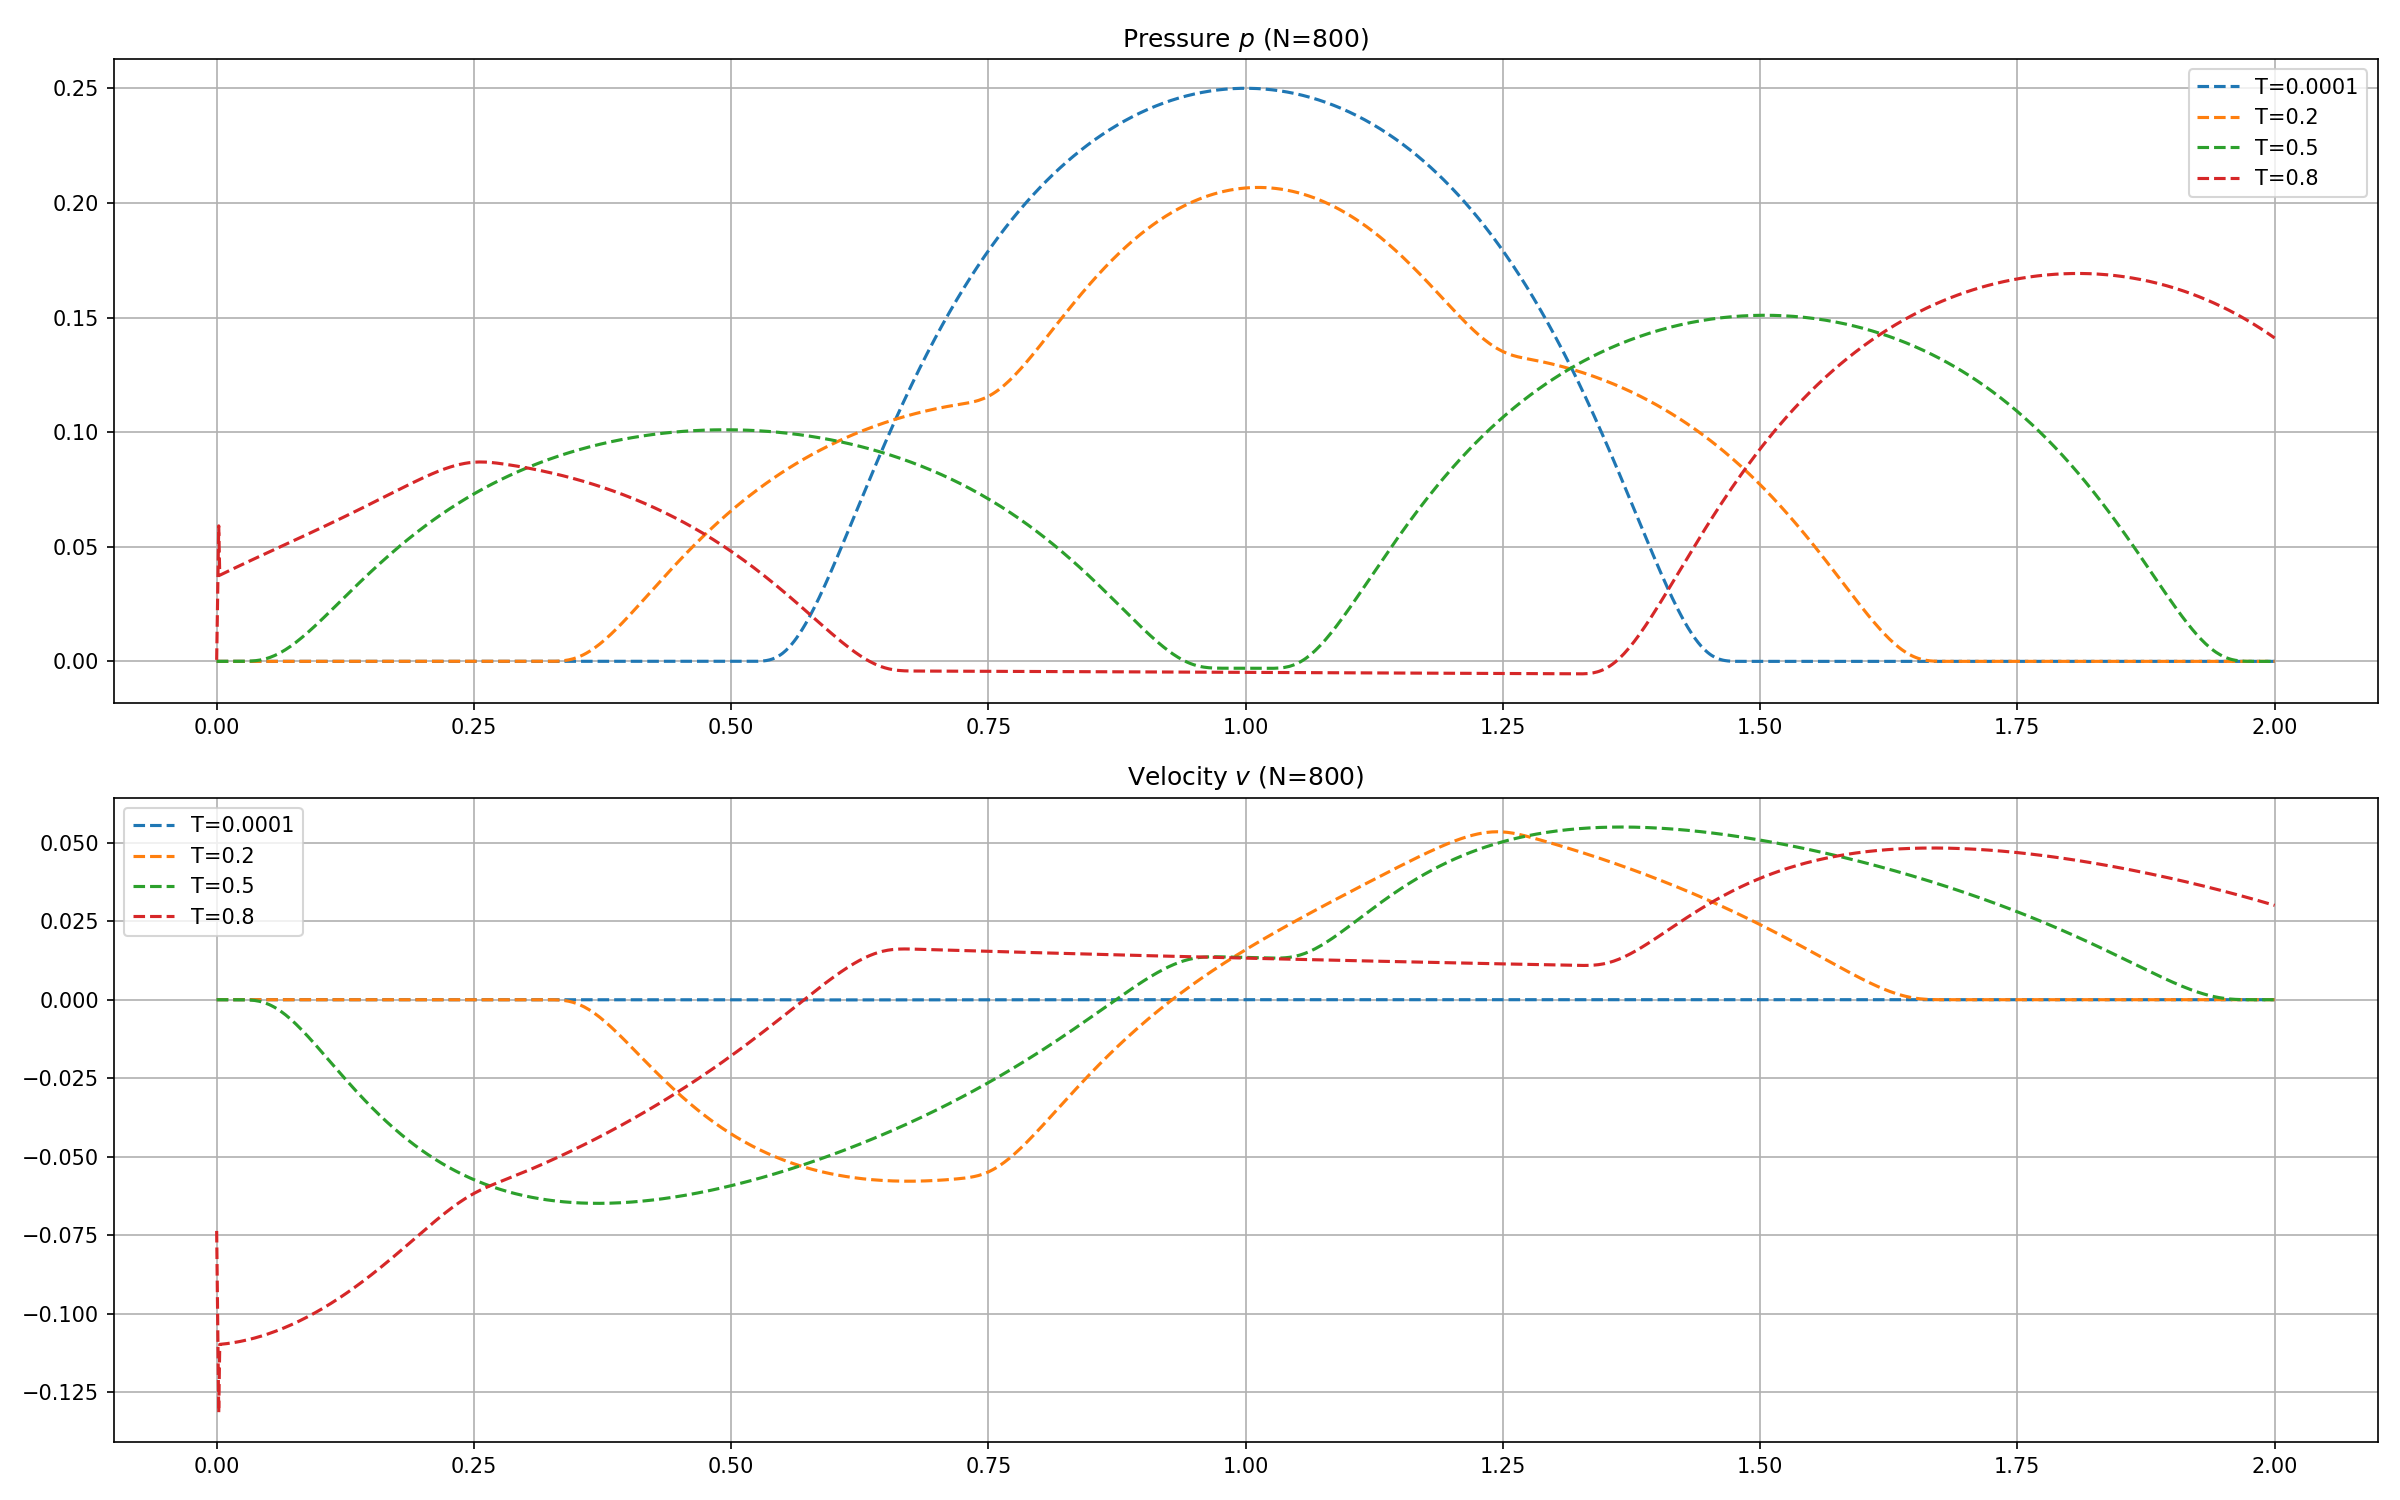
\includegraphics[width=0.65\textwidth]{Images/dg_solution_exp_N800.png}
    \caption{DG numerical solutions exponential cross-section.}
    \label{fig:dg_solution_exp}
\end{figure}
\end{frame}

\slideTitle{Result - Conical Cross-Section}
\begin{figure}[htbp]
    \centering
    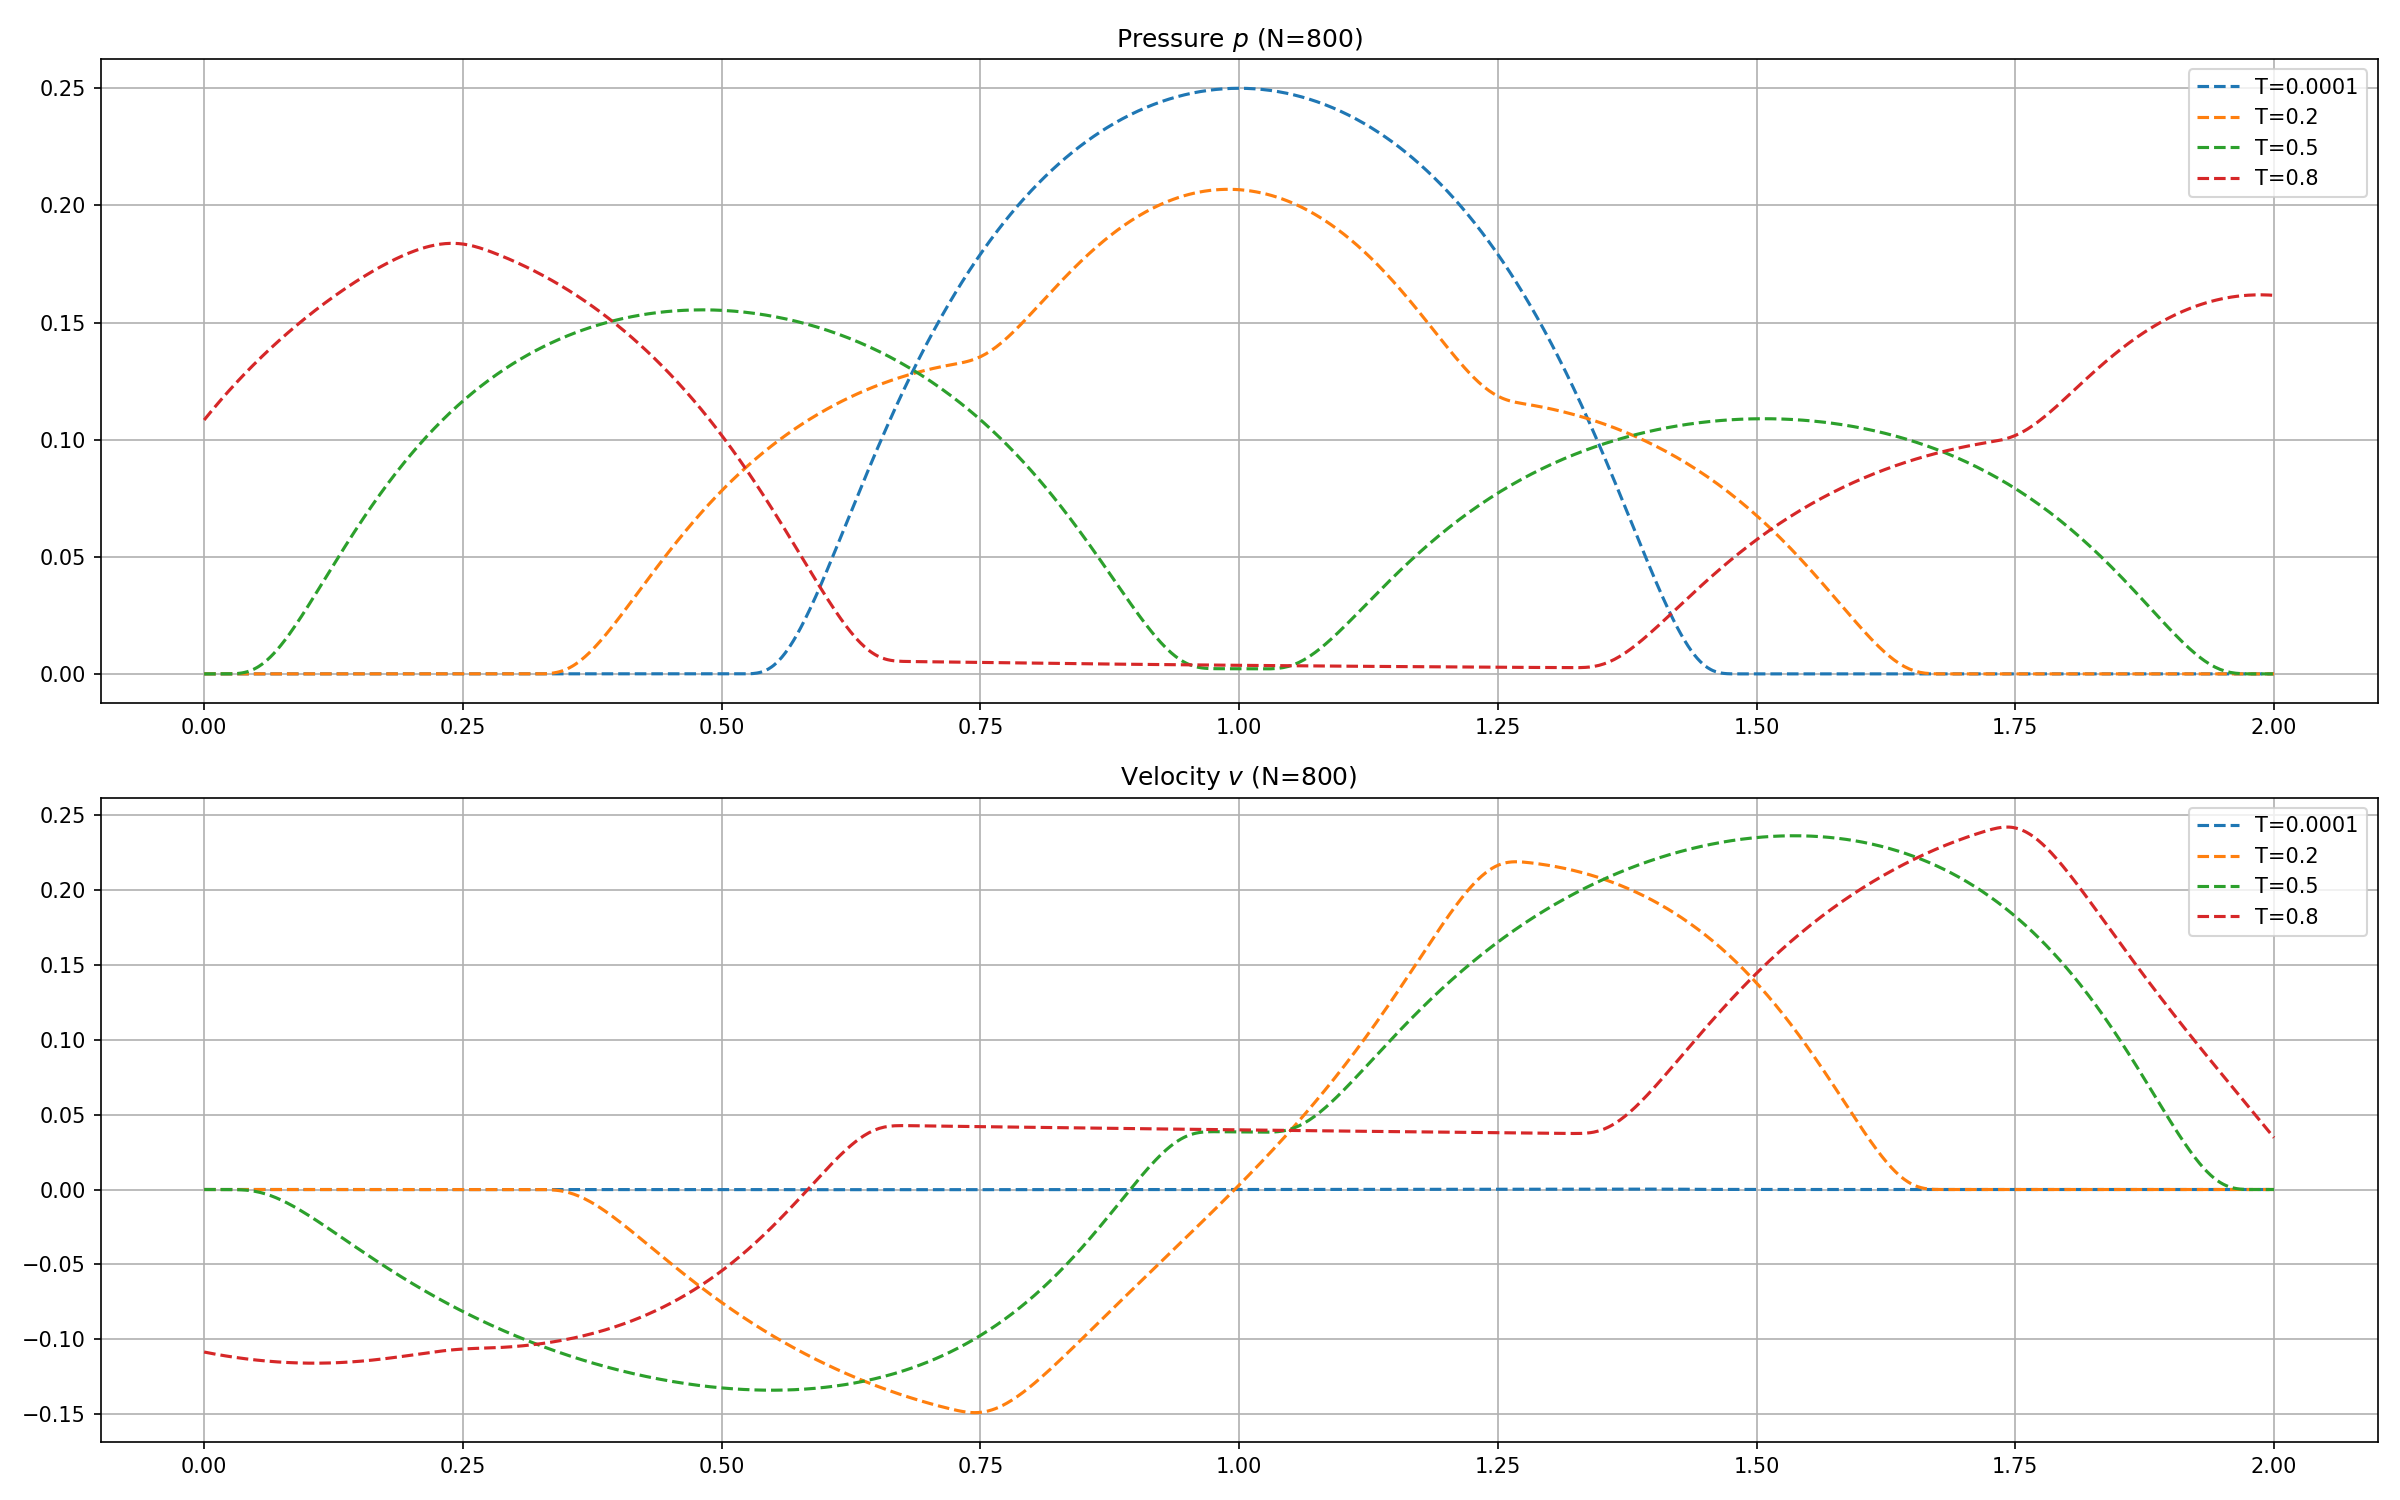
\includegraphics[width=0.65\textwidth]{Images/dg_solution_cone_N800.png}
    \caption{DG numerical solutions conical cross-section.}
    \label{fig:dg_solution_cone}
\end{figure}
\end{frame}

\subsection{Performance Study}
\begin{frame}
\frametitle{Performance Study}

\centering \scriptsize Execution time (s) for different cross-section profiles for Euler explicit and Runge--Kutta 
2 time integration schemes.

\begin{columns}[T]
    \begin{column}{0.5\textwidth}
        \centering
        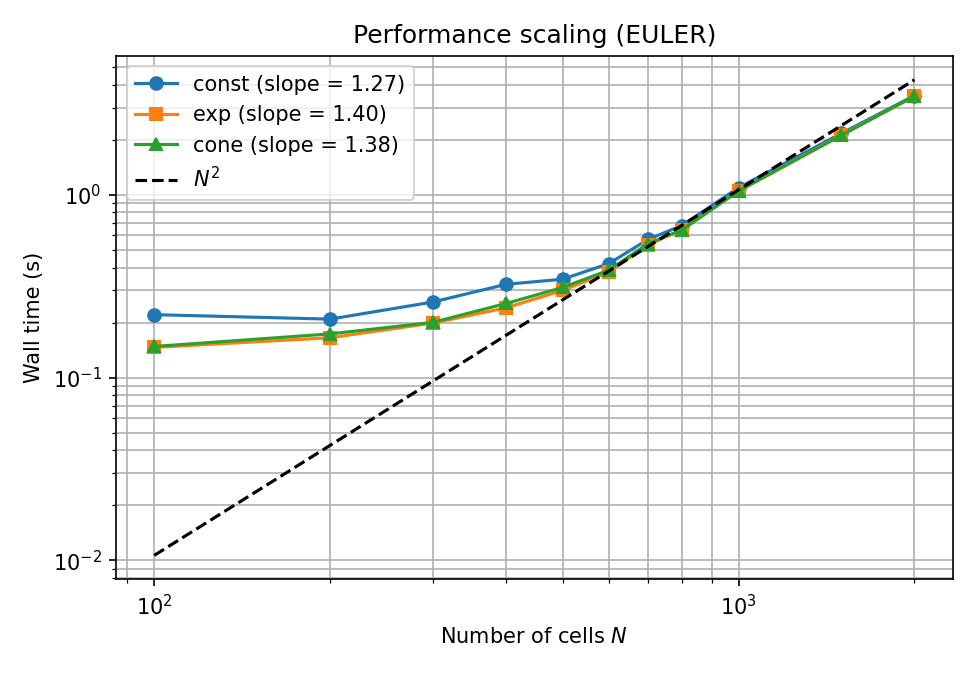
\includegraphics[width=\linewidth]{Images/performance_euler.png}
        \par\smallskip
        \scriptsize (a) Explicit Euler
    \end{column}
    \begin{column}{0.5\textwidth}
        \centering
        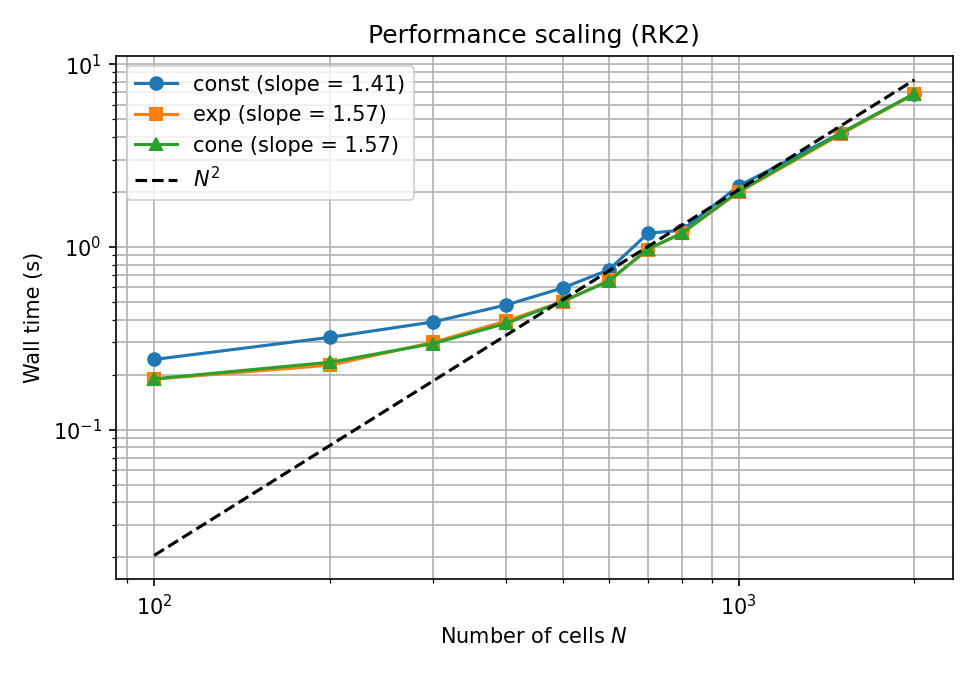
\includegraphics[width=\linewidth]{Images/performance_rk2.png}
        \par\smallskip
        \scriptsize (b) Runge--Kutta 2
    \end{column}
\end{columns}
\par\medskip
\label{fig:execution_time}
\normalsize
For larger $N$, the execution time scales $\sim N^2$, as expected.
\end{frame}
\section{Conclusion}
\slideTitle{Conclusion}

\begin{itemize}
    \item This project focused on the automated calibration of physical parameters
    in a one-dimensional wave model for reed instruments.
    
    \item Key contributions:
    \begin{itemize}
        \item Formulation and implementation of a DG scheme for the mixed wave system with variable cross-section,
        \item Treatment of radiation boundary conditions using characteristic variables
        coupled with a boundary ODE,
        \item Validation against analytical solutions in the constant-section case,
        \item Implementation with Explicit Euler and RK2 time integration schemes.
    \end{itemize}

    \item Numerical results demonstrate accuracy, stability, and expected convergence rates.
    
    \item The JAX-based implementation shows good computational scalability and
    is well suited for future automated calibration tasks.
\end{itemize}
\end{frame}

\slideTitle{Perspectives}
Future work may include:
\begin{itemize}
    \item Compute the conservative form of the mixed wave equations,
    \item Extension to full model by adding LHS boundary conditions,
    \item Investigation of suitable loss functions and training strategies,
    \item Integration into an automated calibration and optimization framework.
\end{itemize}

\vspace{2em}
\textbf{Acknowledgments:} 
\vspace{0.5em}

I would like to express my sincere gratitude to my supervisors\\[0.2em]
\textbf{Dr.\ Emmanuel Franck, Dr.\ Juliette Chabassier, Dr.\ Laurent Navoret,\\
Dr.\ Victor Michel-Dansac, and Dr.\ Alexis Thibault}\\[0.4em]
for their invaluable guidance, insightful discussions, and continuous
support throughout this project.
\end{frame}

\begin{frame}[allowframebreaks]{References}
\printbibliography
\end{frame}

\section{Annexes}
\subsection{Performance Tables}

\slideTitle{Performance Tables}
\begin{columns}[T]
    \begin{column}{0.5\textwidth}
        \centering
        \textbf{Euler explicite}\\[0.5em]
        \begin{table}[h!]
\centering
\begin{tabular}{c ccc}
\hline
$N \backslash S(x)$ & Const. & Exp. & Cone \\
\hline
100 & 0.250 & 0.154 & 0.142 \\
200 & 0.205 & 0.175 & 0.156 \\
300 & 0.238 & 0.213 & 0.198 \\
400 & 0.325 & 0.249 & 0.245 \\
500 & 0.344 & 0.326 & 0.296 \\
600 & 0.409 & 0.387 & 0.371 \\
700 & 0.569 & 0.545 & 0.522 \\
800 & 0.666 & 0.739 & 0.620 \\
1000 & 1.059 & 1.053 & 1.021 \\
1500 & 2.248 & 2.151 & 2.076 \\
2000 & 3.526 & 3.327 & 3.380 \\
\hline
\end{tabular}
\caption{Execution time (s) of the DG P1 solver using the EULER scheme.}
\label{tab:performance-euler}
\end{table}

    \end{column}
    \begin{column}{0.5\textwidth}
        \centering
        \textbf{Runge--Kutta 2}\\[0.5em]
        \begin{table}[h!]
\centering
\begin{tabular}{c ccc}
\hline
$N \backslash S(x)$ & Const. & Exp. & Cone \\
\hline
100 & 0.237 & 0.189 & 0.188 \\
200 & 0.325 & 0.218 & 0.225 \\
300 & 0.386 & 0.280 & 0.298 \\
400 & 0.503 & 0.386 & 0.376 \\
500 & 0.594 & 0.502 & 0.487 \\
600 & 0.720 & 0.639 & 0.624 \\
700 & 0.986 & 0.952 & 0.939 \\
800 & 1.205 & 1.162 & 1.173 \\
1000 & 2.079 & 1.943 & 1.962 \\
1500 & 3.931 & 4.024 & 3.937 \\
2000 & 6.579 & 6.484 & 6.693 \\
\hline
\end{tabular}
\caption{Execution time (s) of the DG P1 solver using the RK2 scheme.}
\label{tab:performance-rk2}
\end{table}

    \end{column}
\end{columns}
\end{frame}

\subsection{Simulation Parameters}

\slideTitle{Simulation Parameters}
\begin{table}[h!]
\centering
\begin{tabular}{c cccccc}
\hline
Parameters & $\alpha$ & $\beta$ & $S^\ast$ & c & $Z^\ast_T$ & CLF \\
\hline
Values & 0.1 & 0.2 & 1 & 1 & 1.0 & 0.05 \\
\hline
\end{tabular}
\caption{Simulation parameters used in the DG P1 solver.}
\label{tab:sim_parameters}
\end{table}
\end{frame}

\subsection{Use of AI Assistance}
\begin{frame}{Use of Artificial Intelligence Assistance}

\small
\begin{itemize}
    \item Some parts of this work were prepared with the assistance of Artificial Intelligence (AI) tools.
    
    \item \textbf{Tool used:}
    \begin{itemize}
        \item \textbf{ChatGPT} (OpenAI, GPT-4 / GPT-5 family)
    \end{itemize}

    \item \textbf{Scope of use:}
    \begin{itemize}
        \item Code support and debugging
        \item Documentation and algorithm reformulation
        \item Bibliography generation
    \end{itemize}

    \item \textbf{Typical prompts included:}
    \begin{itemize}
        \item Argument parsing in Python
        \item Repository structure documentation
        \item \texttt{.bib} file generation
        \item Ghost-cell debugging
        \item CSV $\rightarrow$ \LaTeX{} $\rightarrow$ PDF automation
        \item Physical modeling examples (cross-sections, compact support)
        \item Pertinent commentaries for code
    \end{itemize}

    \item All AI outputs were verified, adapted, and corrected by the authors, who take full responsibility for the scientific integrity of this work.
\end{itemize}

\end{frame}

\end{document}